\documentclass{article}
\usepackage[utf8]{inputenc} %кодировка
\usepackage[T2A]{fontenc}
\usepackage[english,russian]{babel} %русификатор 
\usepackage{mathtools} %библиотека матеши
\usepackage[left=1cm,right=1cm,top=2cm,bottom=2cm,bindingoffset=0cm]{geometry} %изменение отступов на листе
\usepackage{amsmath}
\usepackage{graphicx} %библиотека для графики и картинок
\graphicspath{}
\DeclareGraphicsExtensions{.pdf,.png,.jpg}
\usepackage{subcaption}
\usepackage{pgfplots}
\usepackage{float}
\usepackage{listings}
\lstset{
    language=bash,
    breaklines=true,
    basicstyle=\ttfamily,
    frame=single,
    showstringspaces=false
}

\begin{document}
% НАЧАЛО ТИТУЛЬНОГО ЛИСТА
\begin{center}
    \Large
    Федеральное государственное автономное \\
    образовательное учреждение высшего образования \\ 
    «Научно-образовательная корпорация ИТМО»\\
    \vspace{0.5cm}
    \large
    Факультет программной инженерии и компьютерной техники \\
    Направление подготовки 09.03.04 Программная инженерия \\
    \vspace{1cm}
    \Large
    \textbf{Отчёт по лабораторной работе №4} \\
        По дисциплине «Бизнес логика программных систем» ( семестр 6)\\
    \large
    \vspace{8cm}

    \begin{minipage}{.33\textwidth}
    \end{minipage}
    \hfill
    \begin{minipage}{.4\textwidth}
    
        \textbf{Студент}: \vspace{.1cm} \\
        \ Дениченко Александр P3312\\
        \textbf{Практик}:  \\
        \ Осипов Святослав
    \end{minipage}
    \vfill
Санкт-Петербург\\ 2025 г.
\end{center}
\pagestyle{empty}
% КОНЕЦ ТИТУЛЬНОГО ЛИСТА 
\newpage
\pagestyle{plain}

\section*{Цель работы}
Цель работы - ознакомиться с методами и средствами построения отказоустойчивых решений на базе СУБД Postgres; получить практические навыки восстановления работы системы после отказа.

\section*{Задание}

\begin{itemize}
    \item В качестве хостов использовать одинаковые виртуальные машины.
    \item В первую очередь необходимо обеспечить сетевую связность между ВМ.
    \item Для подключения к СУБД (например, через psql), использовать отдельную виртуальную или физическую машину.
    \item Демонстрировать наполнение базы и доступ на запись на примере не менее, чем двух таблиц, столбцов, строк, транзакций и клиентских сессий.
\end{itemize}

\subsection*{Ход работы}
Создан ведущий сервер, настроены параметры для репликации.
\begin{center}
    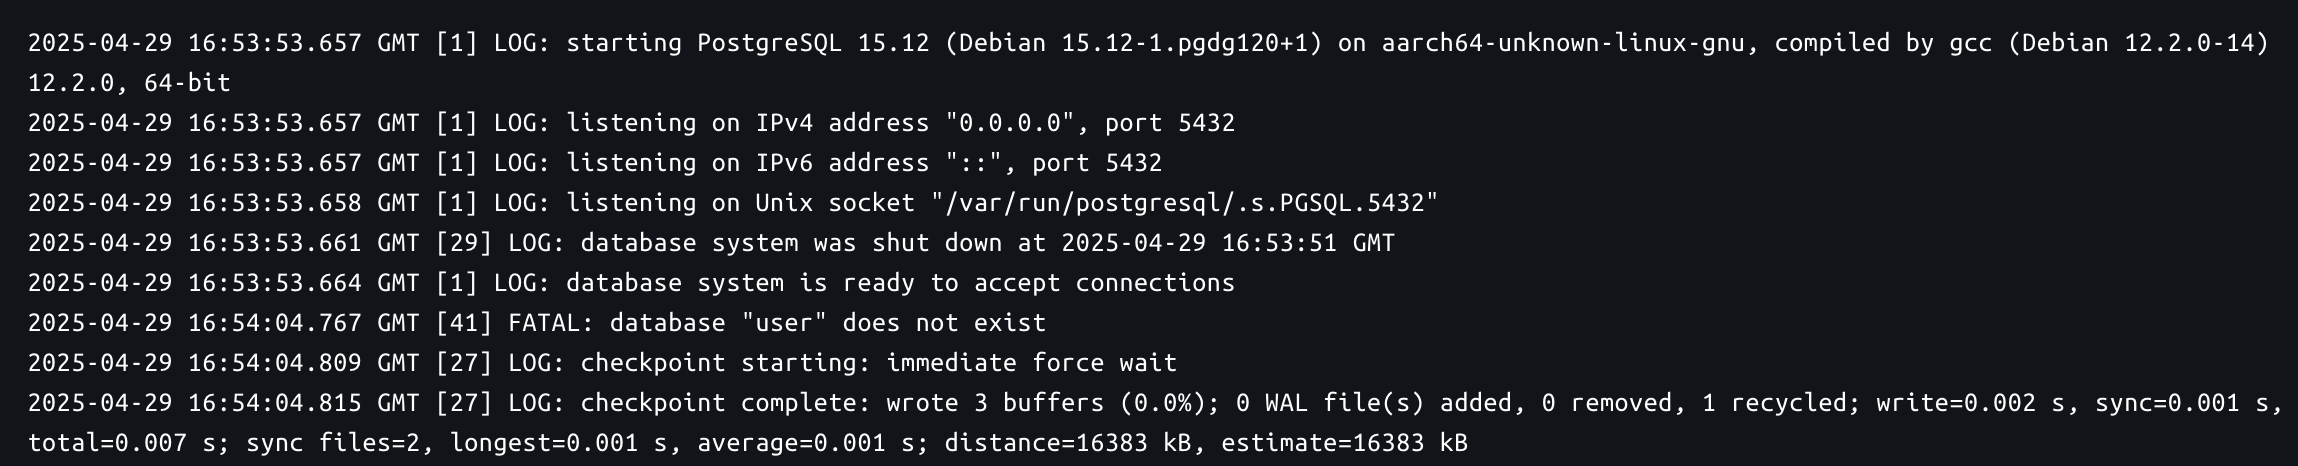
\includegraphics[width=.9\textwidth]{primary.png}
\end{center}
Создан ведомый сервер, настроены параметры для репликации.
\begin{center}
    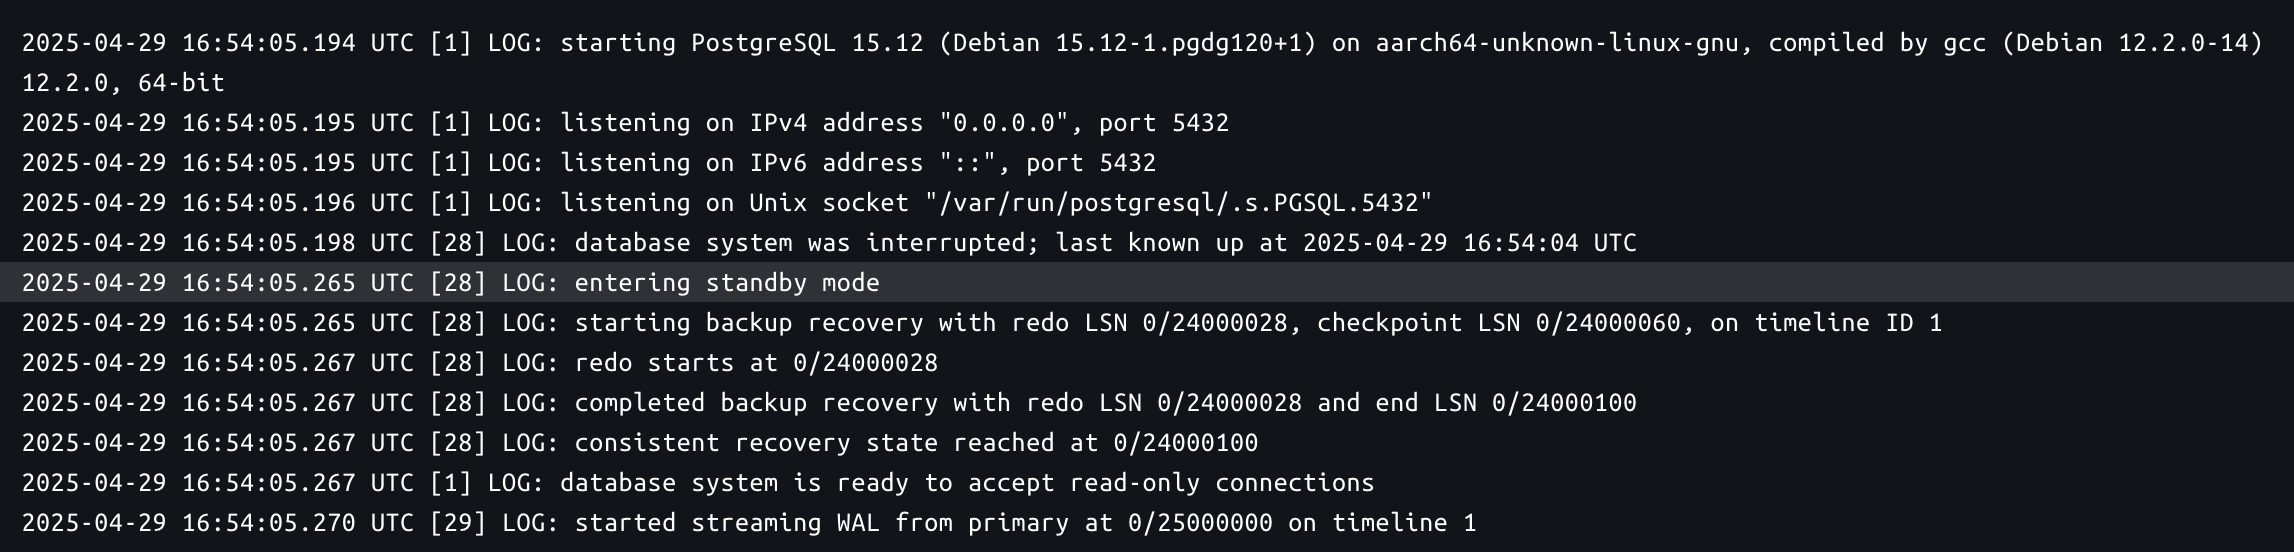
\includegraphics[width=.9\textwidth]{replica.png}
\end{center}
Запросы с хост машины на ведущий сервер.
\begin{center}
    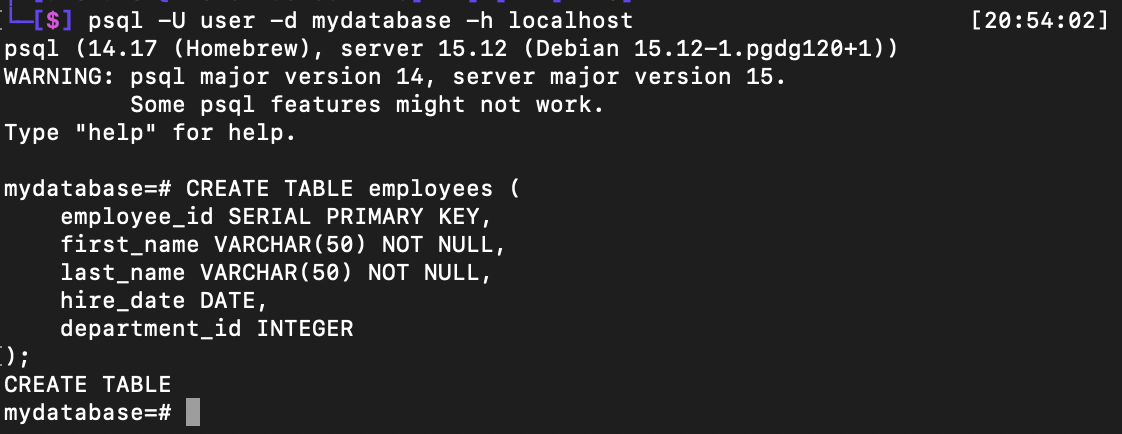
\includegraphics[width=.9\textwidth]{createprimary.png}
\end{center}
\begin{center}
    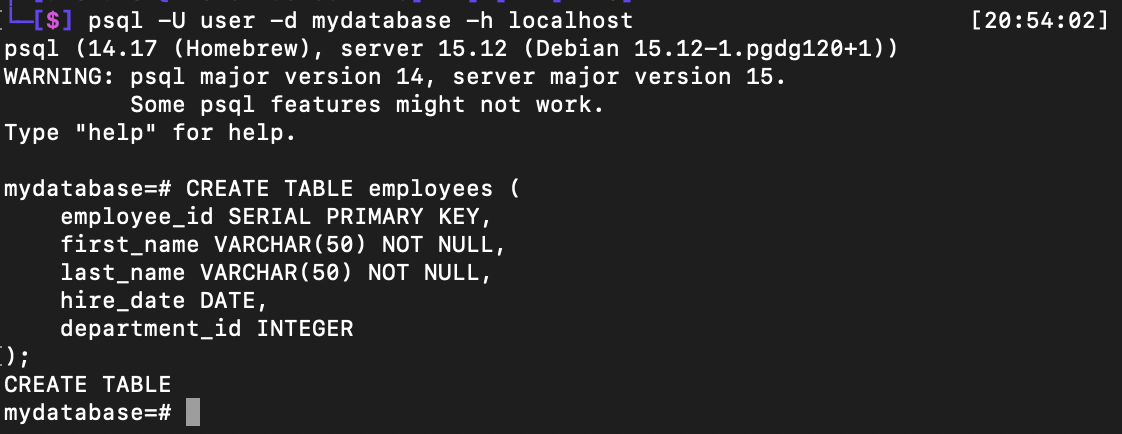
\includegraphics[width=.9\textwidth]{createprimary.png}
\end{center}
\begin{center}
    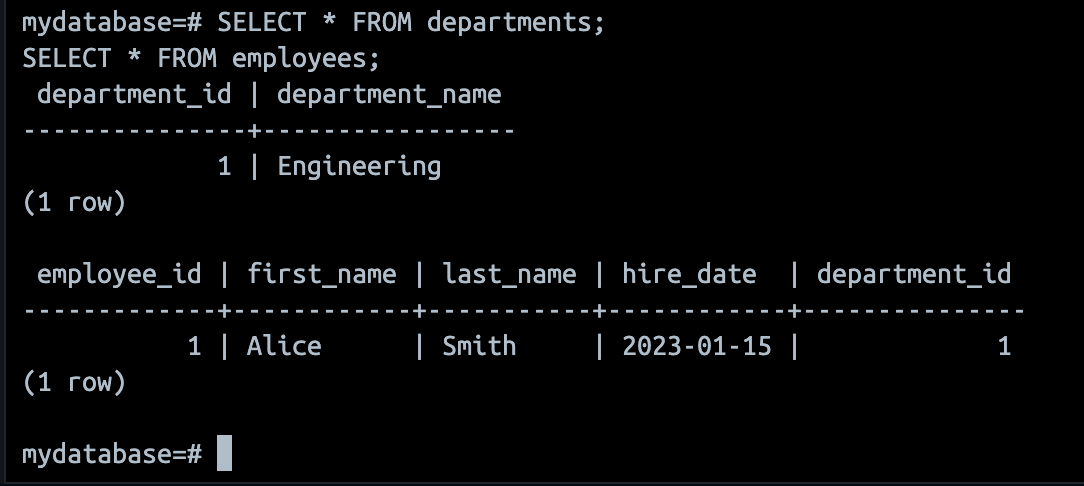
\includegraphics[width=.9\textwidth]{ins-user1.png}
\end{center}
\begin{center}
    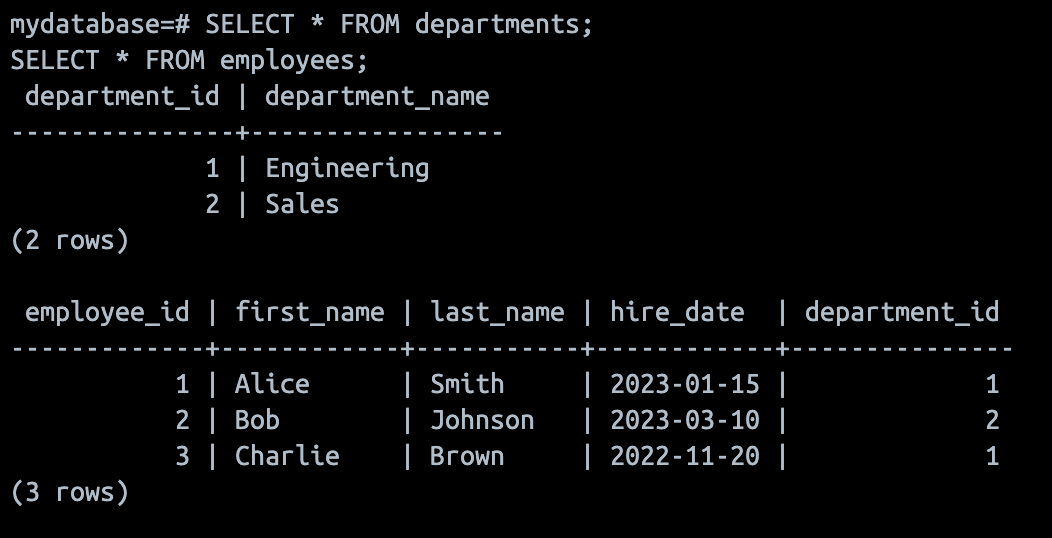
\includegraphics[width=.9\textwidth]{checkprimary.png}
\end{center}

\section*{Эмуляция отказа}
Кладём сервер ведущий.
\begin{center}
    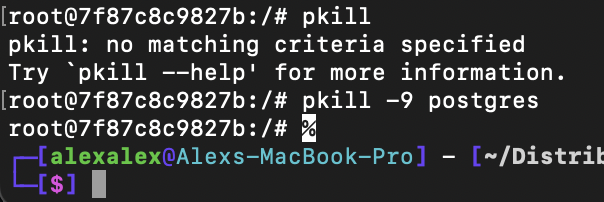
\includegraphics[width=.9\textwidth]{kill.png}
\end{center}
Логи реплики 
\begin{center}
    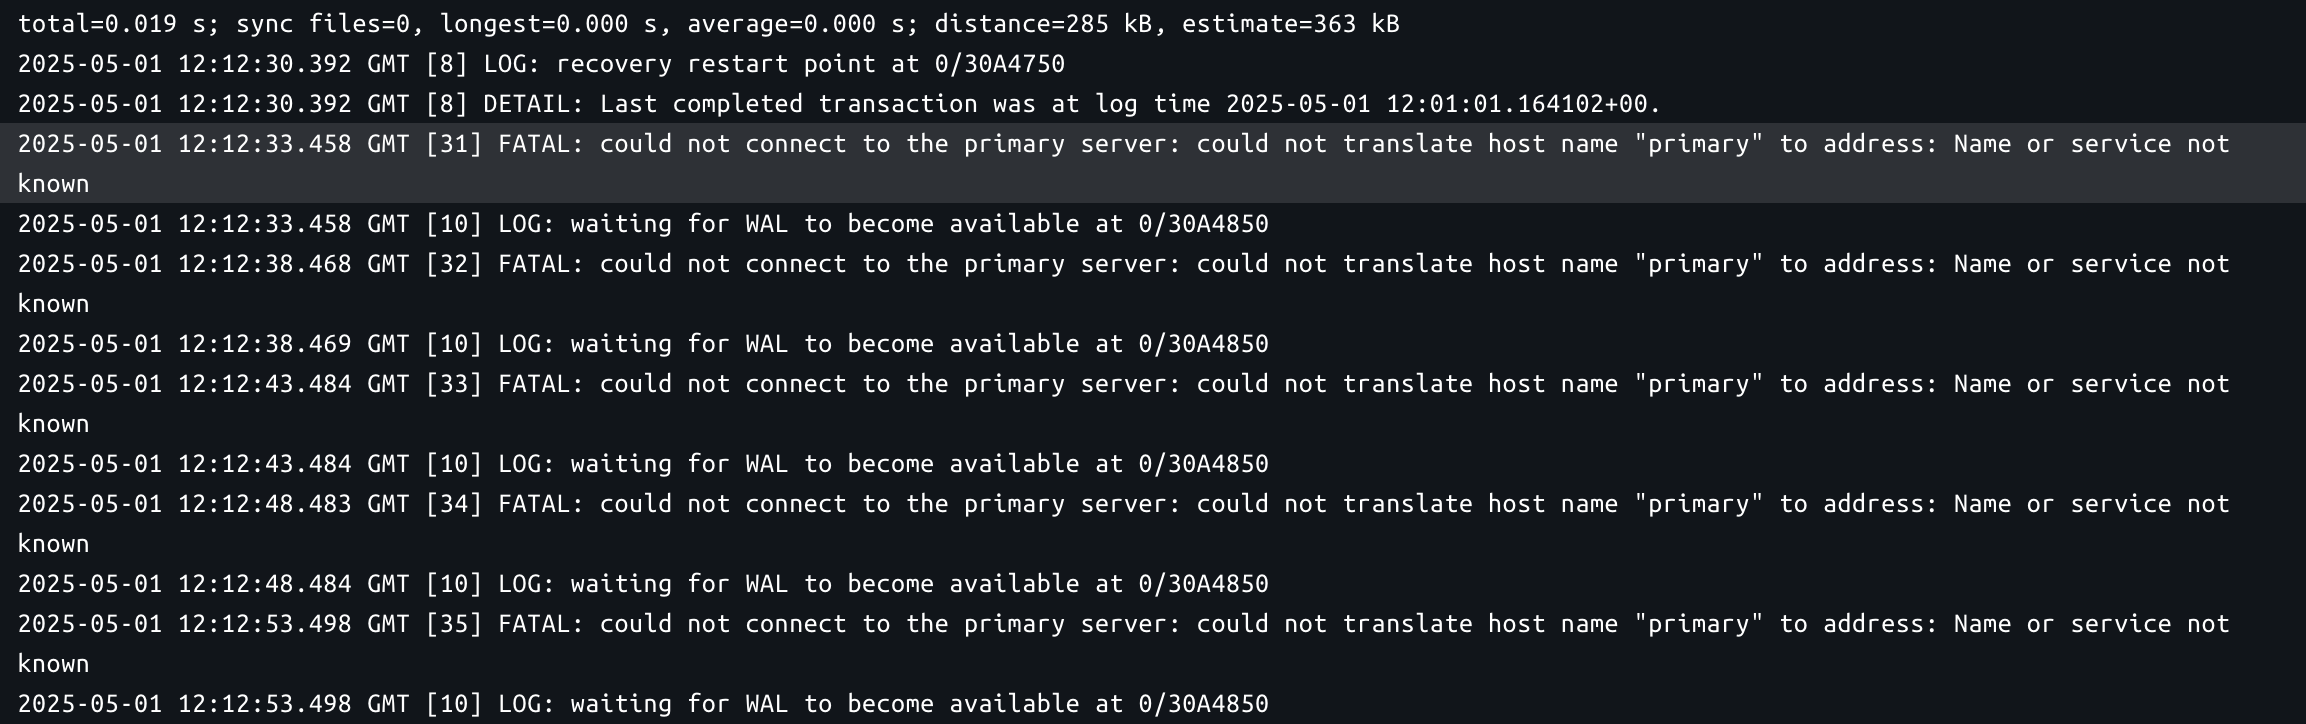
\includegraphics[width=.9\textwidth]{replica-after-kill.png}
\end{center}
Делаем реплику ведущей.
\begin{center}
    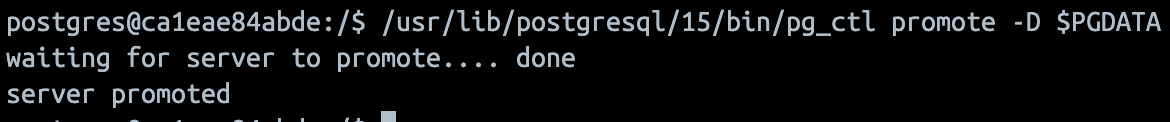
\includegraphics[width=.9\textwidth]{promote.png}
\end{center}
Проверка данных на новом ведущем сервере.
\begin{center}
    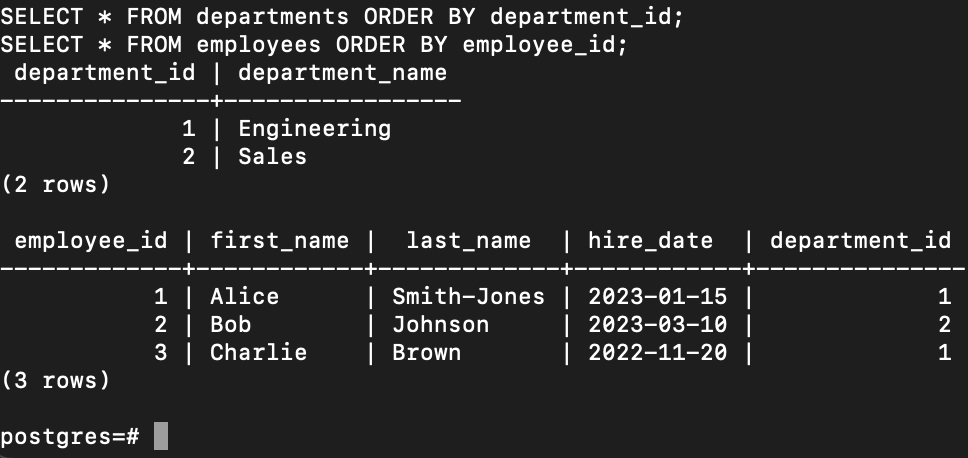
\includegraphics[width=.9\textwidth]{check-promote.png}
\end{center}
Эмуляция работы и изменения данных на новом ведущем сервере.
\begin{center}
    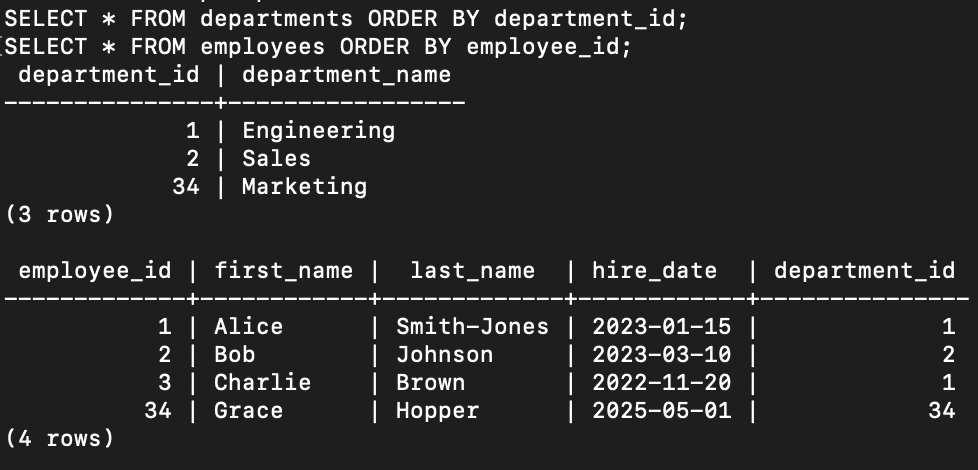
\includegraphics[width=.9\textwidth]{promote-primary.png}
\end{center}

\section*{Восстановление}
Из-за специфика докера, пришлось залезть в volume старого ведущего контейнера через другой временный контейнер и сделать следующие действия. 

(само создание контейнера)
\begin{lstlisting}
    docker run --rm -it --network lab-4_pg_network -v lab-4_pg_primary_data:/var/lib/postgresql/data ubuntu:22.04 bash
    apt-get update && apt-get install -y postgresql-client-15 postgresql-15
    export PGDATA=/var/lib/postgresql/data
    chown -R postgres:postgres $PGDATA
\end{lstlisting}
Удаление старого постмастера
\begin{lstlisting}
    rm -f $PGDATA/postmaster.pid
\end{lstlisting}
Запуск утилиты pg\_rewind, которая сделает старый ведущий сервер ведомым.
\begin{lstlisting}
    su postgres -c "/usr/lib/postgresql/15/bin/pg_rewind --target-pgdata=$PGDATA --source-server='host=replica port=5432 user=postgres dbname=postgres'"
\end{lstlisting}
Создание standby.signal и настройка подключения
\begin{lstlisting}
    touch $PGDATA/standby.signal
    echo "primary_conninfo = 'host=replica port=5432 user=postgres application_name=old_primary'" > $PGDATA/postgresql.auto.conf
\end{lstlisting}
После этих действий можно запускать новый ведущий сервер.
\begin{center}
    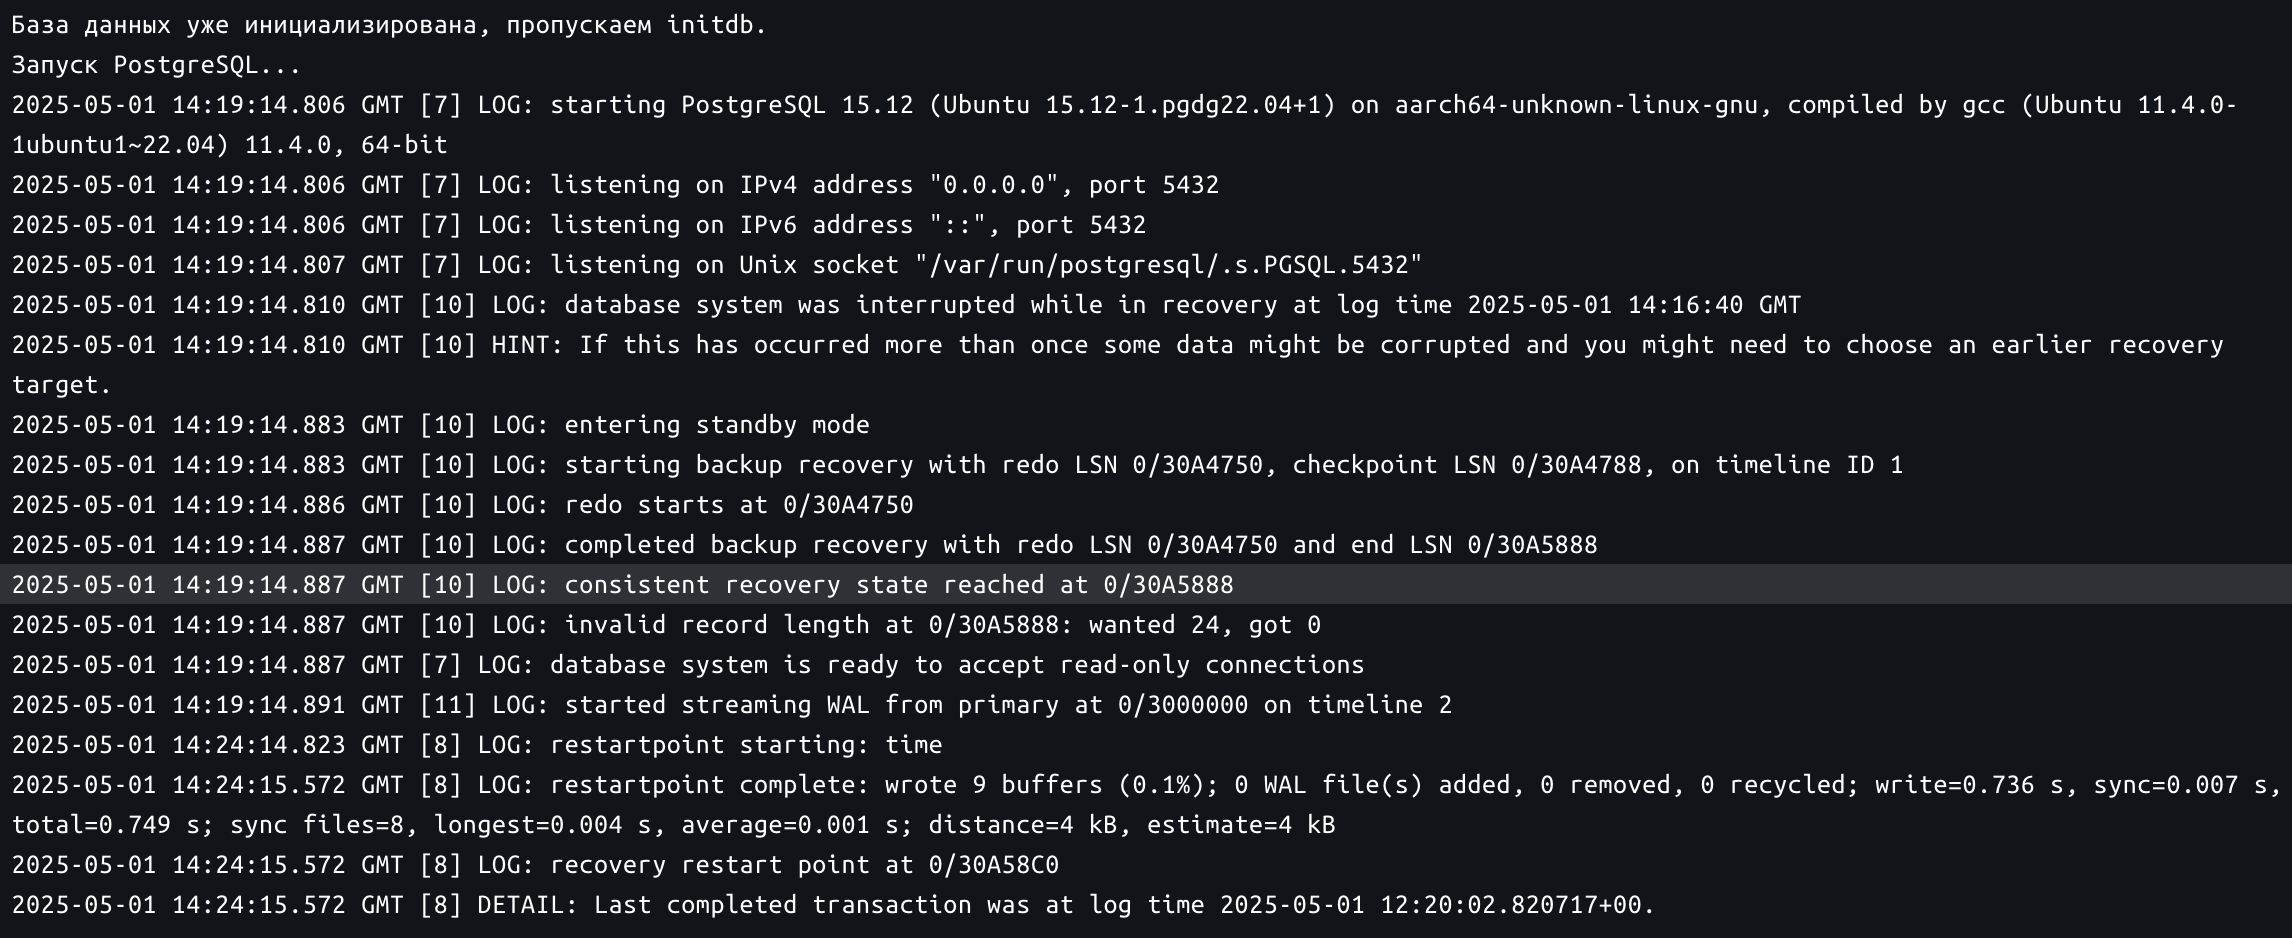
\includegraphics[width=.9\textwidth]{new-replica-logs.png}
\end{center}
\begin{center}
    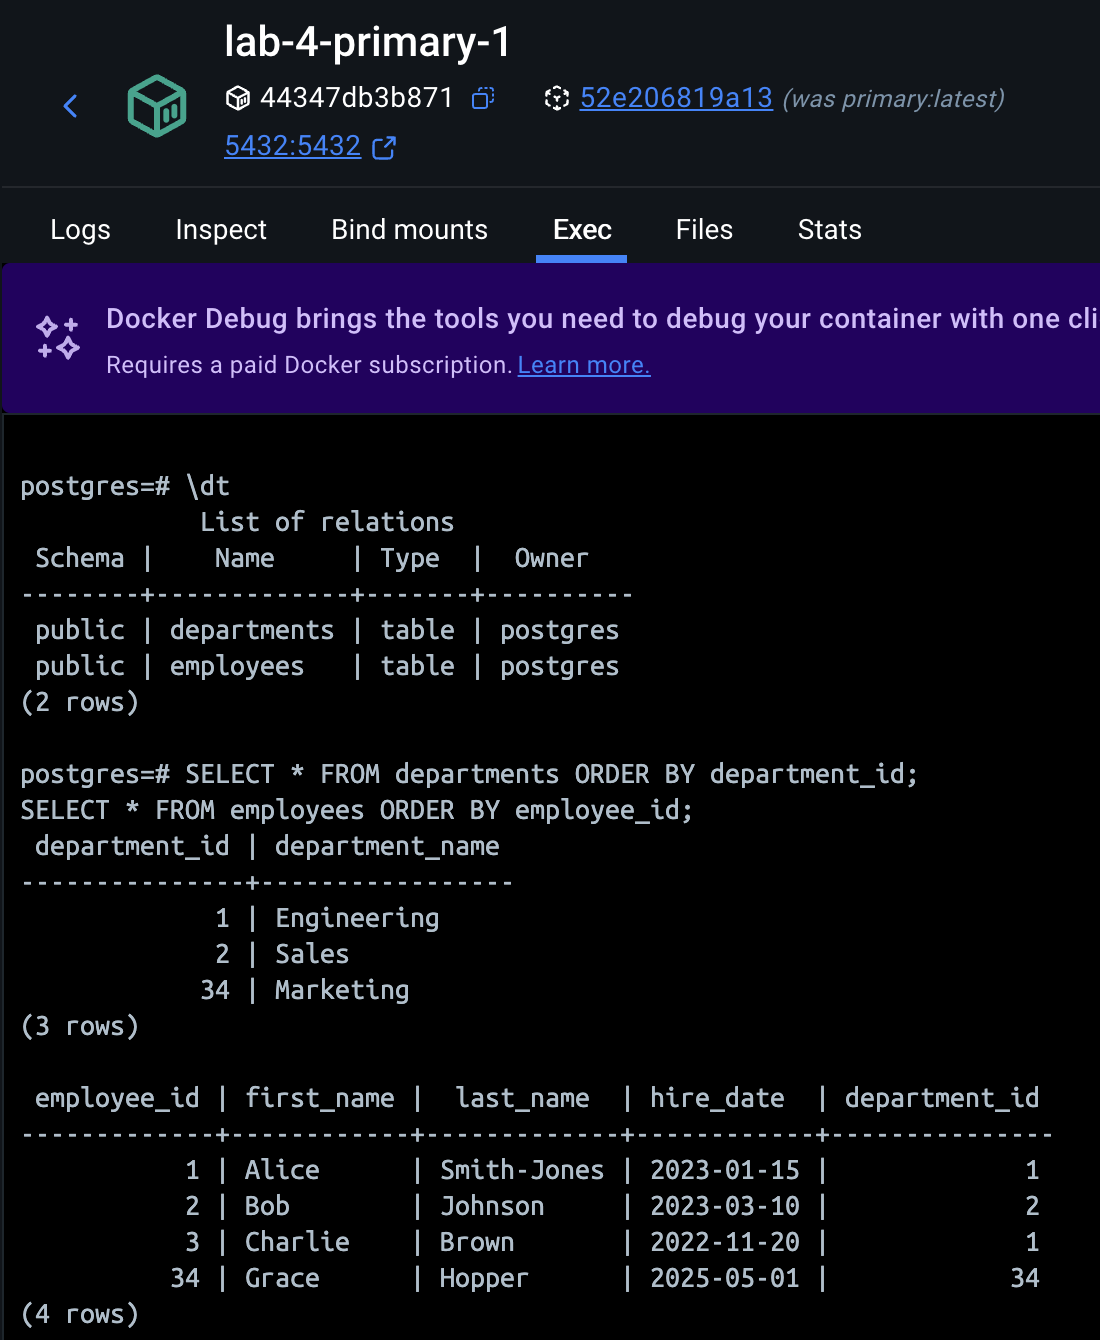
\includegraphics[width=.9\textwidth]{new-replica.png}
\end{center}

\section*{Вывод}
Лабораторная работа была выполнена два раза до момента восстановления, так как в первый раз образ postgres докера не проходил проверку healthcheck. Переписано на чистую ubuntu с полной конфигурацией.


\end{document}
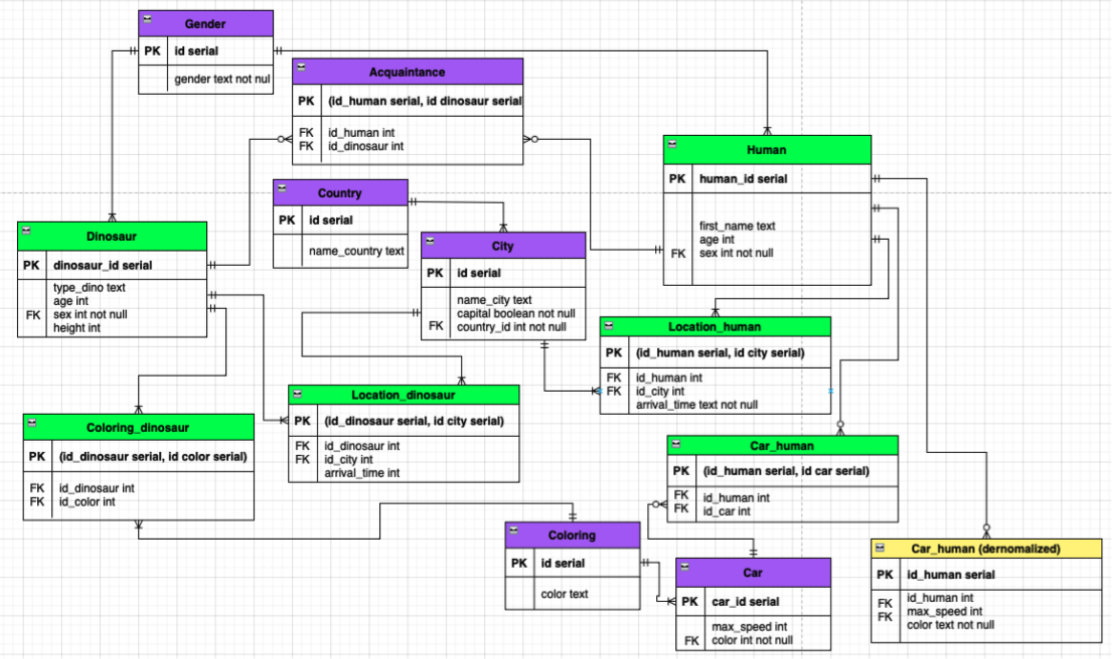
\includegraphics[width=.9\textwidth]{123}